
\section{Introduction}

%\myfirstpara{Gallbladder Cancer (GBC)}
%
%Lately, automated GBC detection has drawn an increased interest from the researchers \cite{basu2022surpassing, basu2023radformer, chang2022ct, kinoshita2023deep}. GBC is difficult to detect at an early stage \cite{howlader2017seer}, and surgical resection becomes infeasible for most patients as the disease gets detected at a late stage. As a result, the disease shows bleak survival statistics. The 5-year survival rate for patients with advanced GBC is only 5\%, and the mean survival time is six months \cite{randi2006gallbladder, gupta2021locally}. Hence, early detection of GBC is crucial for timely intervention and improving the survival rate \cite{hong2014surgical}. %Earlier studies suggest that early detection of GBC can improve the 5-year survival rate significantly \cite{hong2014surgical}.

%\mypara{Ultrasound (USG) for GBC Detection}
%
%USG has been the preferred non-invasive diagnostic imaging modality owing to its low cost, accessibility, and non-ionization. Often, it is the sole imaging performed on patients with abdominal diseases in low-resource countries. However, unlike benign afflictions like stone or polyp, identifying signs of malignancy from routine USG is challenging for radiologists \cite{gupta2020imaging,gb-rads-paper}. GBC may advance silently if it remains undetected. Thus, it is imperative to identify GBC from USG at an early stage. 

\mypara{Motivation}
%
%Detecting GBC from USG images using Deep Neural Networks (DNNs) is challenging. As we have discussed in \Cref{chap:usg}, USG images often have low quality due to sensor issues such as shadows or textures, causing biases in DNNs and making it hard to pinpoint the gallbladder (GB) region accurately. The handheld nature of the probe also means the views are not aligned, adding to the challenge. Malignant cases, unlike the non-malignant one, may not demonstrate clear anatomy due to the presence of lesions. GBC is also difficult to detect due confounding medical conditions. 
Our earlier efforts to circumvent the challenges (earlier discussed in \Cref{sec:challenges}) of USG for accurate GBC detection techniques are primarily image-based. 
Image-centric methodologies demonstrate shortcomings in capturing the intricate representations inherent in video data. Due to the challenges discussed earlier, singular images may lack the requisite features for unambiguous malignancy categorization. Further, due to the operator variability, image-based methods may also exhibit bias due to the frames/ view selected by the radiologists for diagnosis. Image-based techniques exhibit efficacy primarily in small-scale datasets. Our experiments reveal that they fail to generalize effectively to larger, unseen data. 

In response, we argue in favor of a paradigm shift to video-based GBC detection from USG to leverage the rich spatiotemporal information. We employ masked autoencoder-based self-supervised representation learning to discern malignant features from USG video sequences for GBC detection. Notably, video-based GBC detection from USG has not been attempted in the literature. We have earlier explored using videos for contrastive pretraining to enhance the performance of the downstream image-based classifier. However, USG scans are typically available in the form of videos. Radiologists often manually select specific frames that they consider most informative from these videos. From a clinical utility standpoint, predicting directly from the videos would streamline the process and eliminate operator bias introduced by radiologists during the selection of key frames.

\mypara{Masked Autoencoders (MAEs)}
%
Recently, MAEs \cite{adamae, maest, mgmae, videomae, videomaev2} have surfaced as a promising technique for representation learning in vision-centric tasks. 
The concept behind MAE involves masking specific parts, also referred to as tokens, within the input and subsequently attempting to reconstruct these masked segments from the visible components as a pretraining task. Usually, a Vision Transformer (ViT) \cite{vit} generates the embedding of the tokens. Mask sampling strategy plays a significant role in effectively learning using MAEs \cite{maest, videomae}. Currently, a random masking strategy is adopted in most MAE approaches \cite{maest, videomae, videomaev2}. For random masking in videos, patch masking \cite{maest}, frame masking \cite{qian2021spatiotemporal, wei2022masked}, or tube-based masking (dropping tokens at the same spatial location across a few consecutive frames) \cite{videomae} are popularly used. Tube-based masking strategy is considered to be better at preventing information leakage arising from redundancy in the time dimension. %However, studies suggest that a single masking strategy may not fit all datasets due to the diversity of scenes, acquisition conditions, and high/ low spatiotemporal information regions in videos \cite{adamae}. For example, Video-MAE \cite{videomae} achieves the best action classification on the SSv2 dataset  \cite{ssv2} with random tube masking. 
Nevertheless, research indicates that employing a uniform masking strategy may not be universally effective across all datasets, owing to the variability in scenes, acquisition conditions, and the presence of high or low spatiotemporal information regions in videos \cite{adamae}. For instance, Video-MAE demonstrates superior action classification performance on the SSv2 dataset \cite{ssv2} through the utilization of random tube masking. On the other hand, for Kinetics-400 dataset \cite{kinetics}, MAE-ST attains the best performance through random patch masking. \cref{focusmae_fig:teaser_a} shows examples of different masking strategies. 
\begin{figure}[t]
    \centering
    \begin{subfigure}[b]{0.45\linewidth}
        \centering
        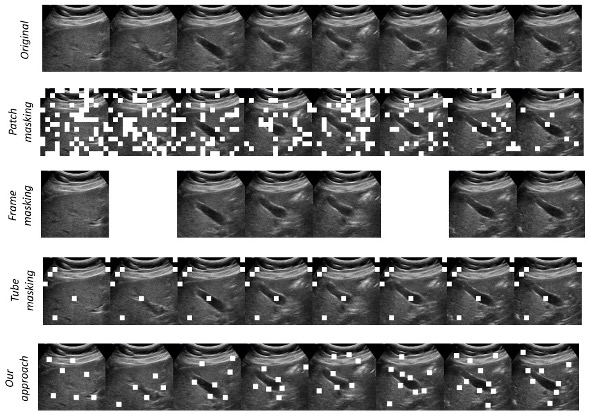
\includegraphics[width=\linewidth]{figs/focusmae/teaser_patch.jpg}
        \caption{}
        \label{focusmae_fig:teaser_a}
    \end{subfigure}
    %
	\begin{subfigure}[b]{0.45\linewidth}
		\centering
		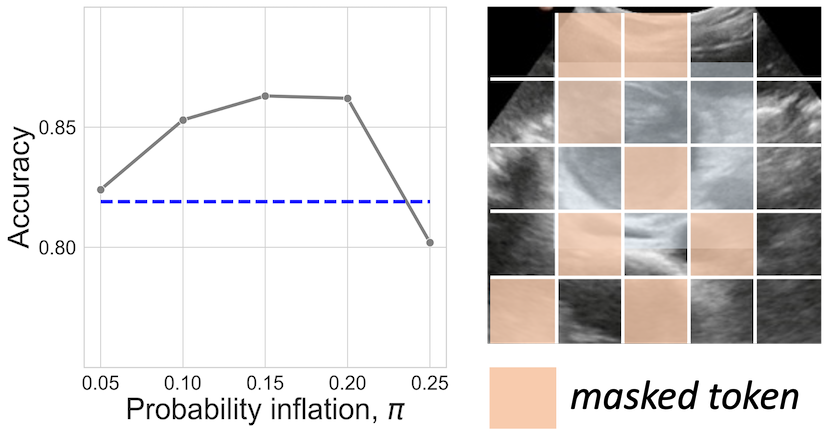
\includegraphics[width=0.95\linewidth]{figs/focusmae/obj_prior.png}
		\caption{}
		\label{focusmae_fig:teaser_b}
	\end{subfigure}
    \caption[Masking strategy of FocusMAE and its motivation]{(a) Masking strategy of FocusMAE in comparison to existing random patch \cite{maest}, frame \cite{wei2022masked}, tube \cite{videomae} masking. Our masking approach selects more tokens from the semantically meaningful regions with a small number of background tokens for masking. (b) Effect of increasing masking probability on object regions. We inflate the masking probability of the tokens which spatially lie within the object region (gray region) by $\pi$. However, excessive masking of the object region degrades performance. The blue line shows the accuracy of the original random masking. }
    \label{focusmae_fig:teaser}
\end{figure}

\mypara{Our Proposal}
%
In USG videos, the spatiotemporal regions indicative of malignancy typically constitute a humble portion. Notice that these are high information regions as opposed to non-GB portions of the frames, which are low information regions. 
Thus, random masking (uniform distribution) is not conducive to learning effective representations of malignancy. The random selection of masked tokens introduces redundant background information, necessitating a more systematic approach. Few recent approaches suggest using an adaptive mask sampling strategy for more meaningful semantic representation \cite{adamae, mgmae}. MGMAE \cite{mgmae} suggests using object motions to guide the mask sampling. AdaMAE \cite{adamae} exploits a policy gradient optimization strategy by the maximization of the expected token reconstruction error in order to boost the sampling probability of the tokens belonging to the objects. Since the organs are mostly stationary in USG videos or CT volumes, the motion-guided strategy is not applicable to our case. On the other hand, our experiments show that AdaMAE does not perform significantly better than VideoMAE. By focusing solely on reconstruction error, the model may underrepresent crucial features or patterns within the data. In contrast, we adopt a simple strategy called \focusmae to effectively mask the high-information patches in the input to learn better disease representation. We identify semantically meaningful candidate high-information regions, and systematically bias the sampling strategy with these region-priors to sample the masking tokens from these focused candidate regions. By using a stronger masking on the high information regions, and reconstructing these tokens, \focusmae learns a more refined representation of GBC. %malignancy. 

\par We validate the \focusmae method on a curated dataset which contains the 64 videos from the GBUSV dataset (refer to \cref{data:gbusv}), and 27 additional malignant videos. Since our idea of focused masking is generic, we validate the generality of the method by applying it to a public CT-based Covid identification task \cite{covidctmd}.

\mypara{Contributions} 
%
The key contributions of this chapter are:
%\vspace{-0.5em}
\begin{enumerate}[label=\textbf{(\arabic*)}]
%\itemsep-0.6em
	\item We posit that existing SOTA techniques for GBC detection in USG images exhibit suboptimal accuracy and generalization performance. Image-centric methodologies demonstrate shortcomings in capturing the intricate representations inherent in video data. Singular images may lack the requisite features for unambiguous malignancy categorization. Consequently, we advocate for a paradigm shift toward video-based GBC detection for USG. 
	%Image-centric methodologies demonstrate shortcomings in capturing the intricate representations inherent in video data. Singular images may lack the requisite features for unambiguous malignancy categorization. Further, image-based techniques exhibit efficacy primarily in small-scale datasets. Our experiments reveal that they fail to generalize effectively to larger, unseen data. In response, we employ masked autoencoder-based representation learning to discern malignant features from USG video sequences for GBC detection.
	%
	\item Even though video-based GBC classification shows improvement over image-based methods in terms of accuracy, specificity, and sensitivity, we observe that the random masking in MAE presents opportunities for further improvement. Notably, the spatiotemporal regions indicative of malignancy typically constitute a small portion of the video. The random selection of masked tokens introduces redundant background information, necessitating a more systematic approach. To address the issue, we propose a novel design, \focusmae, to systematically bias the masking token selection from the semantically meaningful candidate regions. As a result, the network is compelled to learn a more refined representation of GB malignancy while reconstructing the masked tokens. %We report an accuracy of 96.4\% using our approach as against 84\% by the current SOTA of GBCNet \cite{basu2022surpassing} and Radformer \cite{basu2023radformer}\footnote{Both GBCNet and RadFormer gave an identical accuracy in our experiments. We confirmed that individual predictions were not identical.}
	%
	\item Our idea of focused masking is generic, and we validate the generality of the method by applying it to a public CT-based Covid identification task \cite{covidctmd}. %We report an accuracy gain of 2.9\% by our method over the SOTA \cite{videomaev2}.
    %
	%\item Concurrently, we curate the most extensive USG video dataset available for GBC detection. We establish the dataset by adding 27 USG video samples exhibiting GBC to the publicly available GBUSV dataset. The dataset will be made available to the community. 
    %
    %\item We also note that the problem of USG video-centric detection of GBC with machine learning was not previously attempted in literature. We provide the first solution to the problem and present a strong baseline. 
\end{enumerate}
